\documentclass{article} %\usepackage{CJK}
\usepackage{xeCJK}
\usepackage{ctex}
\usepackage{graphicx}
\renewcommand{\contentsname}{目录}
\renewcommand{\abstractname}{摘要}
\author{杨铭 - 5130379022\\
        李晟 - 5130379017\\
        张云翔 - 5130379012}
\title{HCI 课程选题提交}
\begin{document}
\maketitle
\newpage
\section{基于手势的3D建模}
\textbf{李晟 - 5130379017}
\subsection{用户分析}
主要的目标用户是对于三维建模有兴趣的人,年龄段不限。
\subsection{目标}
提供人们一种更加贴近自然的对塑造三维模型的方式,主要包含以下特性:
\begin{itemize}
	\item 可以通过拉、捏、戳等自然动作改变模型的外形。
	\item 可以通过涂抹的方式对模型进行上色。
	\item 支持模型的导入导出。
\end{itemize}
\subsection{创新点}
通过手势识别技术,可以使用户体验到不同于现有的三维建模软件的模型塑造方式。
\subsection{技术需求}
\begin{itemize}
	\item Leap Motion硬件支持
	\item 手势识别算法
	\item 三维模型的顶点编辑和纹理编辑算法
\end{itemize}
\newpage
\section{基于Leap Motion的手势控制魔方音游}
\textbf{杨铭 - 5130379022 \& 李晟 - 5130379017}
\subsection{用户分析}
音游作为较为小众的游戏,受众也不是很大。我们这个想法本质还是一个音游,所以用户群体为广大游戏爱好者特别是音游爱好者。
\subsection{目标}
做出有一定游戏性的通过识别手势进行输入的一个音乐游戏。可能包含以下特性:
\begin{itemize}
  \item 几个自带曲目,可能会有铺面编辑器功能。
  \item 多种基本手势输入法,比如手指滑动,手掌翻动等
  \item 游戏主体是一个魔方,玩家需要按照游戏内的提示给出相应手势来完成合乎音乐节拍的“打击”
\end{itemize}
\begin{figure}[!h]
\begin{minipage}{0.5\linewidth}
%  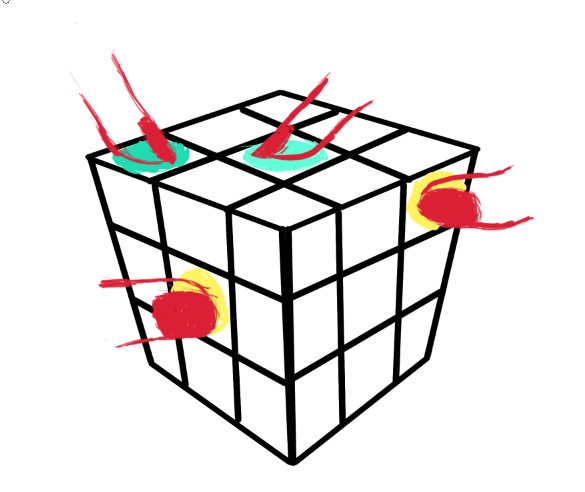
\includegraphics[width=18em]{pic1.png}\\
  \caption{}\label{1-1}
\end{minipage}
\begin{minipage}{0.5\linewidth}
%  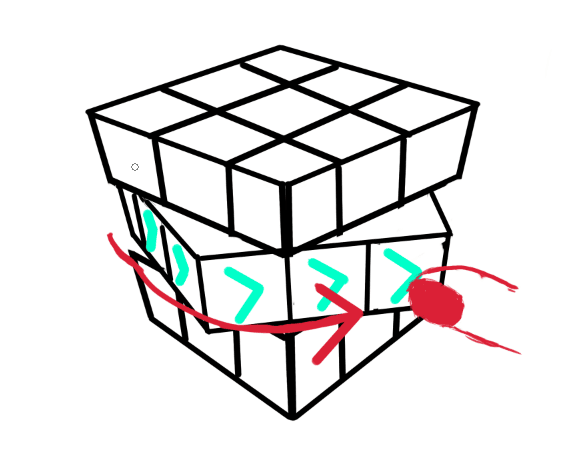
\includegraphics[width=18em]{pic2.png}\\
  \caption{}\label{1-2}
\end{minipage}
\end{figure}

\subsection{创新点}
使用手势操作,革新了传统音乐游戏的玩法。
\subsection{技术支持}
\begin{itemize}
  \item Leap Motion硬件支持
  \item 手势识别
  \item 游戏设计方法
\end{itemize}
\newpage
\section{确认用户起床的闹钟软件}
\textbf{张云翔 - 5130379012}
\subsection{用户分析}
大多数用户在被闹钟叫醒后,难以战胜浓烈的睡意,选择按掉闹钟继续睡眠,这样闹钟的效果没有完全体现出来。这个设计的用户群体为无法通过闹钟有效起床,需要更有效闹钟的用户。
\subsection{目标}
在手机客户端做出一个可以通过用户的物理信息确保用户起床的闹钟
\subsection{创新点}
对于很多人来说,传统的闹钟并不能把人吵醒,而对于那种持续不断的闹钟(例如iphone自带闹钟)只需要触摸手机屏幕就可以停止,用户完全可以先触摸手机屏幕之后再睡觉。实际上,按掉闹钟并不意味着用户已经起床。
我想通过一些辅助手段获取用户的额外信息,来判断用户是否真正起床。
\subsection{技术支持}
\begin{itemize}
  \item 手机传感器
  \item 人体运动识别
\end{itemize}
\end{document}
